\documentclass{standalone}
\usepackage[utf8]{inputenc}

\usepackage{tikz}
\usetikzlibrary{positioning, arrows, fit}
\begin{document}

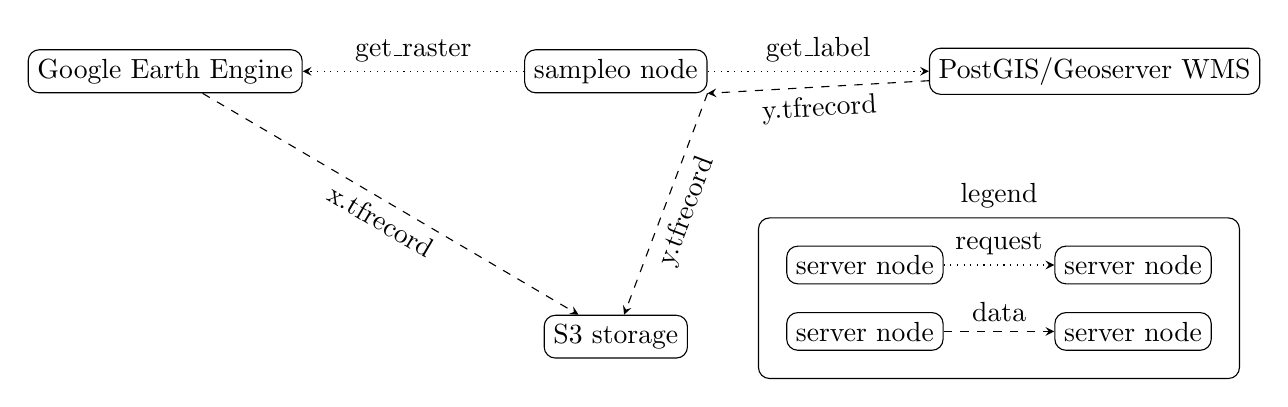
\begin{tikzpicture}[node distance=8em]
	
	\tikzstyle{node}=[draw, rounded corners]
	\tikzstyle{legendbox}=[draw, rounded corners, inner sep=10pt]
    
    \tikzstyle{request}=[-stealth, dotted]
    \tikzstyle{data}=[-stealth, dashed]


	\node[node](sampleo){sampleo node};
    \node[node, right=of sampleo](wms){PostGIS/Geoserver WMS};
    \node[node, below=of sampleo](s3){S3 storage};
    \node[node, left=of sampleo](gee){Google Earth Engine};
    
    \draw[request] (sampleo) -- (gee) node [midway, above] {get\_raster};
    \draw[request] (sampleo) -- (wms) node [midway, above] {get\_label};
    
    \draw[data] (wms) -- (sampleo.south east) node [sloped, midway, below]{y.tfrecord};
    \draw[data] (sampleo.south east) -- (s3)  node [sloped, midway, below]{y.tfrecord};
    \draw[data] (gee) -- (s3) node [sloped, midway, below]{x.tfrecord};
    
    % legend
    \begin{scope}[xshift=9em, yshift=-7em, node distance=1em and 4em]
    \node[node] (legend_serv11) {server node};
    \node[node, right=of legend_serv11] (legend_serv21) {server node};
    
    \draw[request] (legend_serv11) -- (legend_serv21) node [midway, above]{request};
    
    \node[node, below=of legend_serv11] (legend_serv21) {server node};
    \node[node, right=of legend_serv21] (legend_serv22) {server node};
    
    \draw[data] (legend_serv21) -- (legend_serv22) node [midway, above]{data};
    
    \node[legendbox, fit=(legend_serv11)(legend_serv22),label=above:legend]{};
    
    \end{scope}
    
    
\end{tikzpicture}

\end{document}

